%%
%% Copyright 2007, 2008, 2009 Elsevier Ltd
%%
%% This file is part of the 'Elsarticle Bundle'.
%% ---------------------------------------------
%%
%% It may be distributed under the conditions of the LaTeX Project Public
%% License, either version 1.2 of this license or (at your option) any
%% later version.  The latest version of this license is in
%%    http://www.latex-project.org/lppl.txt
%% and version 1.2 or later is part of all distributions of LaTeX
%% version 1999/12/01 or later.
%%
%% The list of all files belonging to the 'Elsarticle Bundle' is
%% given in the file `manifest.txt'.
%%

%% Template article for Elsevier's document class `elsarticle'
%% with numbered style bibliographic references
%% SP 2008/03/01
%%
%%
%%
%% $Id: elsarticle-template-num.tex 4 2009-10-24 08:22:58Z rishi $
%%
%%

%\documentclass[preprint,12pt]{elsarticle}

%% Use the option review to obtain double line spacing
%% \documentclass[preprint,review,12pt]{elsarticle}

%% Use the options 1p,twocolumn; 3p; 3p,twocolumn; 5p; or 5p,twocolumn
%% for a journal layout:
%% \documentclass[final,1p,times]{elsarticle}
%% \documentclass[final,1p,times,twocolumn]{elsarticle}
%% \documentclass[final,3p,times]{elsarticle}
%% \documentclass[final,3p,times,twocolumn]{elsarticle}
%% \documentclass[final,5p,times]{elsarticle}
\documentclass[final,5p,times,twocolumn]{elsarticle}

%% if you use PostScript figures in your article
%% use the graphics package for simple commands
%% \usepackage{graphics}
%% or use the graphicx package for more complicated commands
\usepackage{graphicx}
%% or use the epsfig package if you prefer to use the old commands
%% \usepackage{epsfig}

%% The amssymb package provides various useful mathematical symbols
\usepackage{amssymb}
%% The amsthm package provides extended theorem environments
%% \usepackage{amsthm}

%% The lineno packages adds line numbers. Start line numbering with
%% \begin{linenumbers}, end it with \end{linenumbers}. Or switch it on
%% for the whole article with \linenumbers after \end{frontmatter}.
%% \usepackage{lineno}

%% natbib.sty is loaded by default. However, natbib options can be
%% provided with \biboptions{...} command. Following options are
%% valid:

%%   round  -  round parentheses are used (default)
%%   square -  square brackets are used   [option]
%%   curly  -  curly braces are used      {option}
%%   angle  -  angle brackets are used    <option>
%%   semicolon  -  multiple citations separated by semi-colon
%%   colon  - same as semicolon, an earlier confusion
%%   comma  -  separated by comma
%%   numbers-  selects numerical citations
%%   super  -  numerical citations as superscripts
%%   sort   -  sorts multiple citations according to order in ref. list
%%   sort&compress   -  like sort, but also compresses numerical citations
%%   compress - compresses without sorting
%%
%% \biboptions{comma,round}

% \biboptions{}


\journal{Journal of Chromatography B}

\begin{document}

\begin{frontmatter}

%% Title, authors and addresses

%% use the tnoteref command within \title for footnotes;
%% use the tnotetext command for the associated footnote;
%% use the fnref command within \author or \address for footnotes;
%% use the fntext command for the associated footnote;
%% use the corref command within \author for corresponding author footnotes;
%% use the cortext command for the associated footnote;
%% use the ead command for the email address,
%% and the form \ead[url] for the home page:
%%
%% \title{Title\tnoteref{label1}}
%% \tnotetext[label1]{}
%% \author{Name\corref{cor1}\fnref{label2}}
%% \ead{email address}
%% \ead[url]{home page}
%% \fntext[label2]{}
%% \cortext[cor1]{}
%% \address{Address\fnref{label3}}
%% \fntext[label3]{}

%& SHORT COMMUNICATION about 2850 words 
\title{Multi-omics integrated enrichment analysis and pathway visualization}

%% use optional labels to link authors explicitly to addresses:
%% \author[label1,label2]{<author name>}
%% \address[label1]{<address>}
%% \address[label2]{<address>}

\author[uni]{Lars Rosenbaum}
\author[uni]{Johannes Eichner}
\author[klinikum,dzd]{Rainer Lehmann}
\author[uni]{and Andreas Zell}
\address[uni]{Center for Bioinformatics, University of T\"ubingen, T\"ubingen, Germany}
\address[klinikum]{Division of Clinical Chemistry and Pathobiochemistry (Central Laboratory), University Hospital T\"ubingen, T\"ubingen, Germany}
\address[dzd]{Institute of Diabetes Research and Metabolic Diseases, Member of the German Center for Diabetes Research, University of T\"ubingen, T\"ubingen, Germany}



\begin{abstract}
%% Text of abstract

\end{abstract}

\begin{keyword}
%% keywords here, in the form: keyword \sep keyword
Metabolomics \sep Transcriptomics \sep Proteomics \sep Multi-omics \sep Enrichment analysis \sep Pathway visualization
%% MSC codes here, in the form: \MSC code \sep code
%% or \MSC[2008] code \sep code (2000 is the default)

\end{keyword}

\end{frontmatter}

%%
%% Start line numbering here if you want
%%
% \linenumbers

%% main text
\section{Introduction}
Today, high-throughput methods for the analysis of biological systems, such as microarrays, next generation sequencing, and mass spectrometry generate a wealth of 'omics'-scale data. To develop hypotheses about a biological process or a disease state, a variety of omics-platforms for measuring different genomic, proteomic, and metabolic features are combined in one experimental setup. Probably the most prominent genomic feature is messenger RNA (mRNA), which can be measured by gene expression chips (microarrays) or next generation sequencing techniques. Other important genomic features include microRNA (miRNA), single-nucleotide polymorphisms, and epigenetic information, such as the promoter methylation status (DNAm). The proteomic features include abundance profiling of particular protein isoforms and modifications, such as methylation and phosphorylation. Furthermore, modern mass spectrometry platforms are able to detect and measure the relative intensity of thousands of metabolites with high accuracy. The sensible and integrated visualization of 'omics'-scale data at different levels of abstraction is crucial to obtain biological insight without being overwhelmed by the intrinsic complexity of the data \cite{Gehlenborg2010}. A key concept for representing a change in the state of a biological system are pathway-based visualizations.

A plethora of tools were developed for the inspection of data from individual platforms (see \cite{Gehlenborg2010} for examples). Furthermore, solutions for the combined visualization of transcriptomics (mRNA) and metabolomics data exist \cite{Garcia-Alcalde2011,Waegele2012}. Both Paintomics \cite{Garcia-Alcalde2011} and MassTRIX \cite{Waegele2012} are web-service based tools that are able to visualize mRNA microarray and identified metabolomics data in KEGG \cite{Kanehisa2006} pathways. MassTRIX is able to handle unidentified metabolic data by comparing a mass against theoretical adducts stored in metabolomics databases. An example of a tool that can handle several heterogeneous types of 'omics'-data is the commercial Ingenuity Pathway analysis software (www.ingenuity.com). To date, most available high-level analysis tools are either not freely available or focused on certain specialized platforms and thus not able to perform an integrated analysis of many different types of heterogeneous data. However, complex interactions between multiple layers of gene regulation can only be inferred by the integration of omics datasets across multiple platforms, which requires novel analysis tools with appropriate visualizations.

In this contribution we present a new version of InCroMAP \cite{Wrzodek2012a,Wrzodek2012b}, a standalone Java software which was originally designed for the enrichment analysis and pathway-based visualization of genomic and proteomic data, where multiple biological layers were monitored in the same set of samples. The original version supports the integrated analysis of heterogeneous genomic and epigenomic features, such as mRNA, miRNA, and DNAm, as well as abundance profiles of protein modifications. Furthermore, InCroMAP can import data from any platform that contains expression values that can be either associated to a certain gene or a genomic region. The application was developed to provide a high ease of use. Consequently, all information required, for example, for the mapping between different entity identifiers or the annotation of miRNA with mRNA targets, is either directly included in the tool or dynamically downloaded in the background. In the new version of InCroMAP, we also support the enrichment analysis and pathaway-based visualization of annotated metabolomics data. The tool can import data annotated with some common metabolic database identifier (e.g. HMDB \cite{Wishart2009}) or automatically recognize common compound or IUPAC names. METABOLIC OVERVIEW FEATURE

InCroMAP is freely available under the LGPL3 license at http://www.cogsys.cs.uni-tuebingen.de/software/InCroMAP, including a comprehensive user’s guide and several example files.

\begin{figure*}
\center
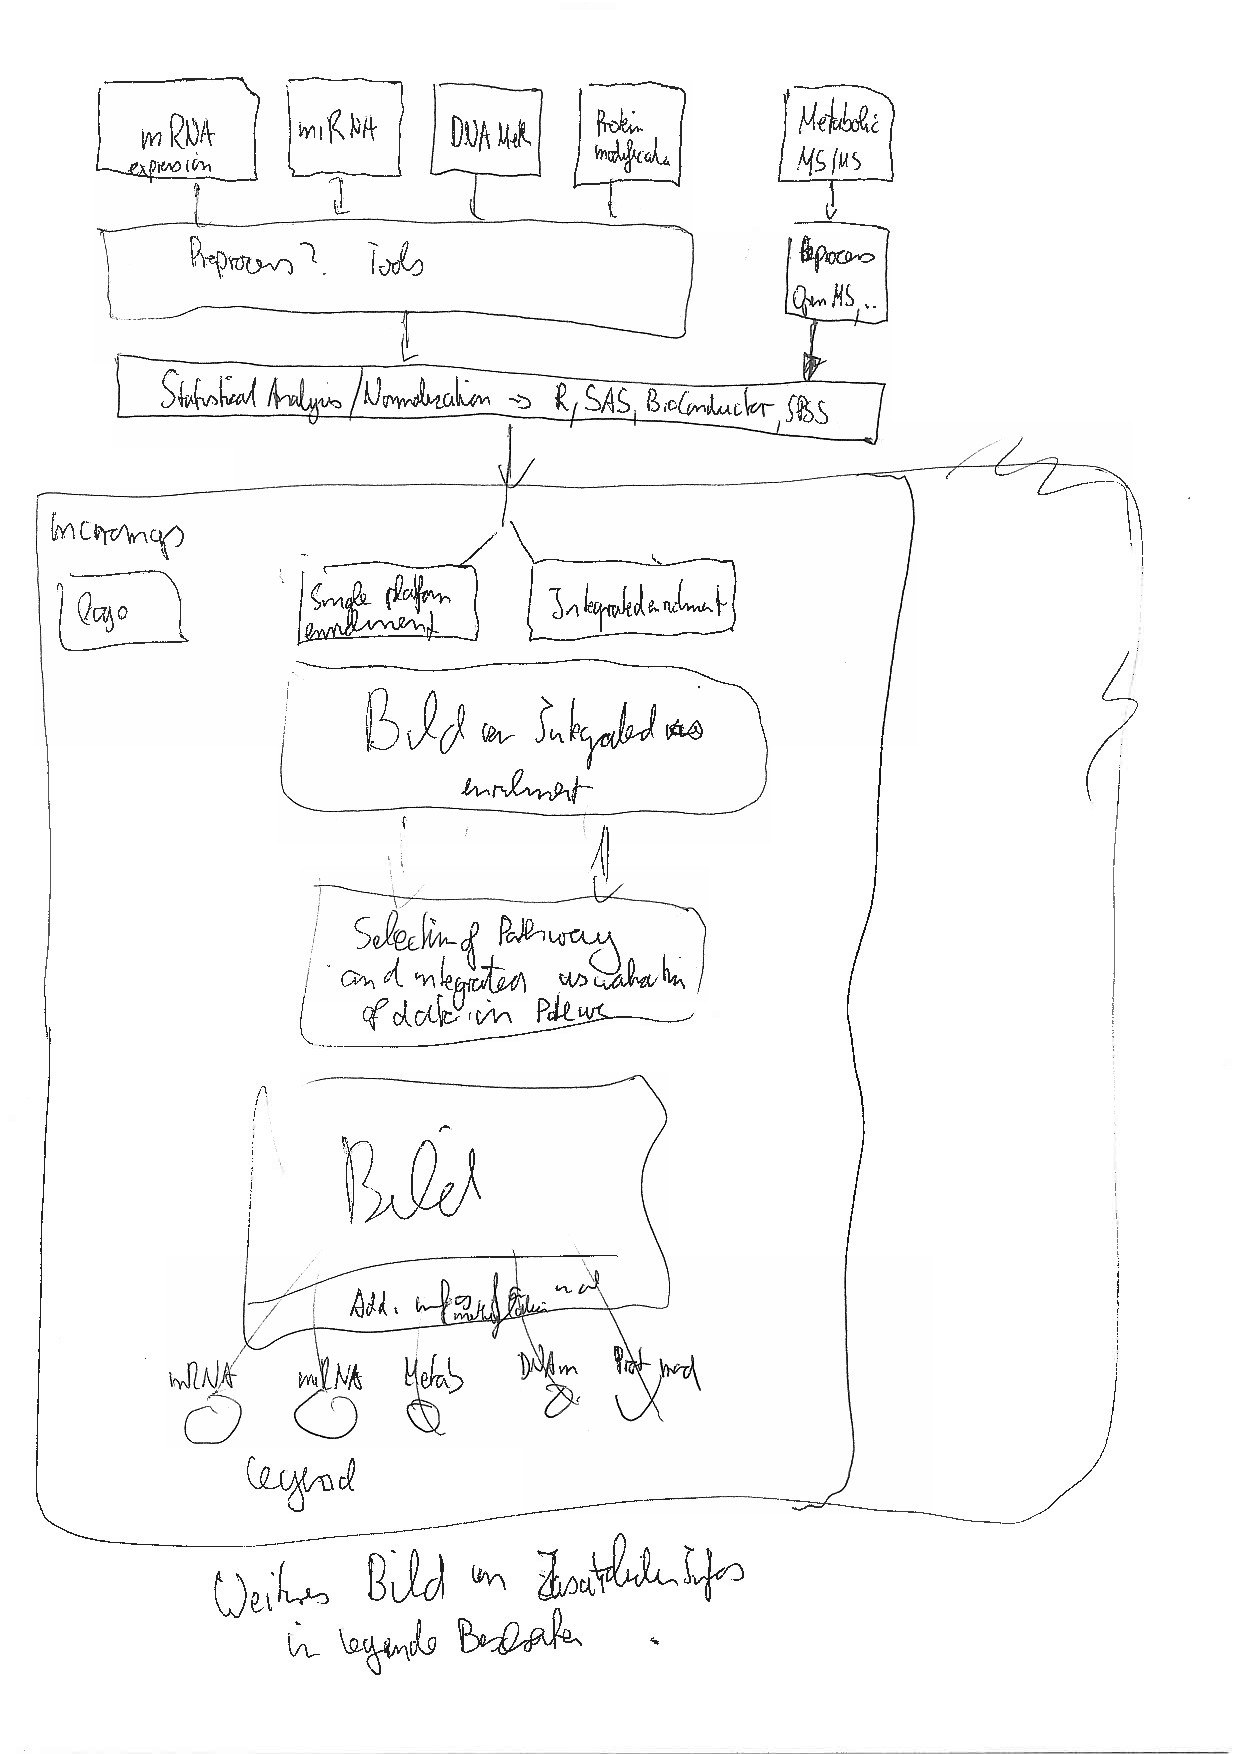
\includegraphics[width=0.9\textwidth]{incromap_overview.pdf}
\caption{\textbf{Overview of typical data analysis workflow}. Da sieht man halt wie geil InCroMAP ist...}
\label{fig:incromap-overview}
\end{figure*}

\section{Methods}
DISCUSS PREPROCESSING OF DATA WITH R AND OpenMS \cite{Sturm2008}.
In a typical use case of InCroMAP the user first imports his preprocessed multi-level omics data, given in tabular format. Then, the deregulated genes for each platform are determined based on appropriate cutoffs and relevant pathways related to the biological background of the experiments are inferred. For this purpose, InCroMAP employs a special pathway enrichment algorithm which integrates deregulated genes across multiple platforms. The resulting pathways can then be selected for further visual inspection from a table in which each pathway is associated with a significance value (see Figure FIGUREb). Alternatively, the metabolic overview function of InCroMAP can be used to generate an interactive global map of cellular metabolism, in which each subordinate metabolic pathway is colored according to the significance of its enrichment with deregulated genes (see Figure XXb). 

\subsection{Visualization of transcriptomics and proteomics data}
In addition to the automatic recognition of identifiers used by the most common oligonucleotide microarray manufacturers (e.g., Affymetrix, Agilent, etc.), we support generic formats to enable the import of processed omics data, provided that each measurement can be either associated to a certain gene or genomic region. Pathways of interest can then either be automatically downloaded from KEGG or imported from other sources in BioPAX format. Being rendered in an interactive graph viewer, the pathway nodes (i.e., genes) can be overlaid with expression data from mRNAs and multiple protein products. Additionally, miRNAs can be connected to a given pathway based on experimentally confirmed or predicted interactions to their target mRNAs. If desired, the tool also visualizes differential methylation of proximal gene promoters, which is by default computed based on the largest peak observed in the upstream region of the transcription start site.

\subsection{Visualization of metabolomics data}
database identifiers , such as PubChem \cite{Wang2009}, HMDB \cite{Wishart2009}, KEGG \cite{Kanehisa2006}, or LIPID MAPS \cite{Sud2007},
\section{Results}

\section{Discussion}
Future extensions: automatic mapping on adducts
improvement of enrichment with many-to-many models
future databases lipidmaps\cite{Sud2007} and reactome \cite{Eustachio2011}
%% The Appendices part is started with the command \appendix;
%% appendix sections are then done as normal sections
%% \appendix

%% \section{}
%% \label{}

%% References
%%
%% Following citation commands can be used in the body text:
%% Usage of \cite is as follows:
%%   \cite{key}         ==>>  [#]
%%   \cite[chap. 2]{key} ==>> [#, chap. 2]
%%

%% References with bibTeX database:

\bibliographystyle{elsarticle-num}
\bibliography{literature}

%% Authors are advised to submit their bibtex database files. They are
%% requested to list a bibtex style file in the manuscript if they do
%% not want to use elsarticle-num.bst.

%% References without bibTeX database:

% \begin{thebibliography}{00}

%% \bibitem must have the following form:
%%   \bibitem{key}...
%%

% \bibitem{}

% \end{thebibliography}


\end{document}

%%
%% End of file `elsarticle-template-num.tex'.
